\documentclass[a4paper, 14pt]{extarticle}

% Поля
%--------------------------------------
\usepackage{geometry}
\geometry{a4paper,tmargin=2cm,bmargin=2cm,lmargin=3cm,rmargin=1cm}
%--------------------------------------


%Russian-specific packages
%--------------------------------------
\usepackage[T2A]{fontenc}
\usepackage[utf8]{inputenc}
\usepackage[english, main=russian]{babel}
%--------------------------------------

\usepackage{textcomp}

% Красная строка
%--------------------------------------
\usepackage{indentfirst}
%--------------------------------------


%Graphics
%--------------------------------------
\usepackage{graphicx}
\graphicspath{ {./images/} }
\usepackage{wrapfig}
%--------------------------------------

% Полуторный интервал
%--------------------------------------
\linespread{1.3}
%--------------------------------------

%Выравнивание и переносы
%--------------------------------------
% Избавляемся от переполнений
\sloppy
% Запрещаем разрыв страницы после первой строки абзаца
\clubpenalty=10000
% Запрещаем разрыв страницы после последней строки абзаца
\widowpenalty=10000
%--------------------------------------

%Списки
\usepackage{enumitem}

%Подписи
\usepackage{caption}

%Гиперссылки
\usepackage{hyperref}

\hypersetup {
	unicode=true
}

%Рисунки
%--------------------------------------
\DeclareCaptionLabelSeparator*{emdash}{~--- }
\captionsetup[figure]{labelsep=emdash,font=onehalfspacing,position=bottom}
%--------------------------------------

\usepackage{tempora}

%Листинги
%--------------------------------------
\usepackage{listings}
\lstset{
  basicstyle=\ttfamily\footnotesize,
  %basicstyle=\footnotesize\AnkaCoder,        % the size of the fonts that are used for the code
  breakatwhitespace=false,         % sets if automatic breaks shoulbd only happen at whitespace
  breaklines=true,                 % sets automatic line breaking
  captionpos=t,                    % sets the caption-position to bottom
  inputencoding=utf8,
  frame=single,                    % adds a frame around the code
  keepspaces=true,                 % keeps spaces in text, useful for keeping indentation of code (possibly needs columns=flexible)
  keywordstyle=\bf,       % keyword style
  numbers=left,                    % where to put the line-numbers; possible values are (none, left, right)
  numbersep=5pt,                   % how far the line-numbers are from the code
  xleftmargin=25pt,
  xrightmargin=25pt,
  showspaces=false,                % show spaces everywhere adding particular underscores; it overrides 'showstringspaces'
  showstringspaces=false,          % underline spaces within strings only
  showtabs=false,                  % show tabs within strings adding particular underscores
  stepnumber=1,                    % the step between two line-numbers. If it's 1, each line will be numbered
  tabsize=2,                       % sets default tabsize to 8 spaces
  title=\lstname                   % show the filename of files included with \lstinputlisting; also try caption instead of title
}
%--------------------------------------

%%% Математические пакеты %%%
%--------------------------------------
\usepackage{amsthm,amsfonts,amsmath,amssymb,amscd}  % Математические дополнения от AMS
\usepackage{mathtools}                              % Добавляет окружение multlined
\usepackage[perpage]{footmisc}
%--------------------------------------

%--------------------------------------
%			НАЧАЛО ДОКУМЕНТА
%--------------------------------------

\begin{document}

%--------------------------------------
%			ТИТУЛЬНЫЙ ЛИСТ
%--------------------------------------
\begin{titlepage}
\thispagestyle{empty}
\newpage


%Шапка титульного листа
%--------------------------------------
\vspace*{-60pt}
\hspace{-65pt}
\begin{minipage}{0.3\textwidth}
\hspace*{-20pt}\centering

\includegraphics[width=\textwidth]{emblem}
\end{minipage}
\begin{minipage}{0.67\textwidth}\small \textbf{
\vspace*{-0.7ex}
\hspace*{-6pt}\centerline{Министерство науки и высшего образования Российской Федерации}
\vspace*{-0.7ex}
\centerline{Федеральное государственное автономное образовательное учреждение }
\vspace*{-0.7ex}
\centerline{высшего образования}
\vspace*{-0.7ex}
\centerline{<<Московский государственный технический университет}
\vspace*{-0.7ex}
\centerline{имени Н.Э. Баумана}
\vspace*{-0.7ex}
\centerline{(национальный исследовательский университет)>>}
\vspace*{-0.7ex}
\centerline{(МГТУ им. Н.Э. Баумана)}}
\end{minipage}
%--------------------------------------

%Полосы
%--------------------------------------
\vspace{-25pt}
\hspace{-35pt}\rule{\textwidth}{2.3pt}

\vspace*{-20.3pt}
\hspace{-35pt}\rule{\textwidth}{0.4pt}
%--------------------------------------

\vspace{1.5ex}
\hspace{-35pt} \noindent \small ФАКУЛЬТЕТ\hspace{80pt} <<Информатика и системы управления>>

\vspace*{-16pt}
\hspace{47pt}\rule{0.83\textwidth}{0.4pt}

\vspace{0.5ex}
\hspace{-35pt} \noindent \small КАФЕДРА\hspace{50pt} <<Теоретическая информатика и компьютерные технологии>>

\vspace*{-16pt}
\hspace{30pt}\rule{0.866\textwidth}{0.4pt}

\vspace{11em}

\begin{center}
\Large {\bf Лабораторная работа № 4} \\
\large {\bf по курсу <<Численные методы линейной алгебры>>} \\
\large <<Метод Крылова поиска собственных значений и векторов>>
\end{center}\normalsize

\vspace{8em}


\begin{flushright}
  {Студент группы ИУ9-72Б Старовойтов А. И. \hspace*{15pt}\\
  \vspace{2ex}
  Преподаватель Посевин Д. П.\hspace*{15pt}}
\end{flushright}

\bigskip

\vfill


\begin{center}
\textsl{Москва 2025}
\end{center}
\end{titlepage}
%--------------------------------------
%		КОНЕЦ ТИТУЛЬНОГО ЛИСТА
%--------------------------------------

\renewcommand{\ttdefault}{pcr}

\setlength{\tabcolsep}{3pt}
\newpage
\setcounter{page}{2}

\section{Задание}\label{Sect::task}

Реализовать метод Крылова для симметричной матрицы. Выполнить проверку
корректности.

\section{Реализация}\label{Sect::impl}

Исходный код программы представлен в листингах~\ref{lst:code1}--~\ref{lst:code7}.

\begin{figure}[!htb]
\begin{lstlisting}[language={},caption={Метод Крылова},label={lst:code1}]
using Test
using Random
using LinearAlgebra

Random.seed!(42)

generate_symmetric_matrix(n) = begin
    A = rand(n, n)
    A = A + A'
    return A
end

is_symmetric(A) = begin
    return A == A'
end

@test is_symmetric(generate_symmetric_matrix(5))

get_B(A, i) = begin
    n = size(A, 1)
    B = Matrix{Float64}(I, n, n)
    for j in 1:n
        if j != i-1
            B[i-1, j] = - A[i, j] / A[i,i-1]
        end
    end
    B[i-1, i-1] = 1/A[i, i-1]
    return B
end

get_frobenius_matrix(A) = begin
    n = size(A, 1)
    D = copy(A)
    B_res = Matrix{Float64}(I, n, n)
    for row in n:-1:2
        if D[row, row-1] == 0
            m = row-2
            while m > 0 && D[row, m] == 0
                m -= 1
            end
            if m == 0
                error("")
            end
            D[:, [m, row-1]] = D[:, [row-1, m]]
            D[m, :], D[row-1, :] = D[row-1, :], D[m, :]
        end
        B = get_B(D, row)

        C = D * B
        D = B \ C
        B_res = B_res * B
    end
    return D, B_res
end

\end{lstlisting}
\end{figure}

% \newpage

\begin{figure}[!htb]
\begin{lstlisting}[language={},caption={Метод Крылова (продолжение)},label={lst:code2}]
@test get_frobenius_matrix([2.2 1.0 0.5 2.0; 1.0 1.3 2.0 1.0; 0.5 2.0 0.5 1.6; 2.0 1.0 1.6 2.0]) == ([6.0 0.20000000000000182 -12.735000000000005 2.7616; 1.0 0.0 0.0 0.0; -1.6037505170817941e-18 1.0 1.1456124527020951e-17 -8.040135925636728e-18; 2.115006742527263e-17 -1.121575634346075e-16 0.9999999999999999 1.4384720710653878e-16], [-0.23112480739599386 1.078582434514638 1.6510015408320498 -1.1587057010785826; 0.081243871690713 -0.1367138254657515 -1.6409581173833871 -0.2739095111360136; 0.2381285894382967 -1.2627819022272029 -0.41315310267544514 0.3695755708082368; 0.0 0.0 0.0 1.0])

find_gershgorin_intervals(A) = begin
    n = size(A, 1)
    intervals = Tuple{Float64, Float64}[]
    for i in 1:n
        interval = (A[i, i] - sum(abs(A[i, j]) for j in 1:n if j != i), A[i, i] + sum(abs(A[i, j]) for j in 1:n if j != i))
        push!(intervals, interval)
    end
    return intervals
end

@test find_gershgorin_intervals([-2.0 0.5 0.5; -0.5 -3.5 1.5; 0.8 -0.5 0.5]) == [(-3.0, -1.0), (-5.5, -1.5), (-0.8, 1.8)]

find_polynom_roots(coeffs, intervals) = begin
    eval_poly(x) = begin
        result = coeffs[1]
        for i in 2:lastindex(coeffs)
            result = result * x + coeffs[i]
        end
        return result
    end

    sorted_intervals = sort(intervals, by = x -> x[1])
    merged = Tuple{Float64, Float64}[sorted_intervals[1]]
    for (a, b) in sorted_intervals[2:end]
        last_a, last_b = merged[end]
        if a <= last_b
            merged[end] = (last_a, max(b, last_b))
        else
            push!(merged, (a, b))
        end
    end
    roots = Float64[]
    tol = 1e-5
    max_iter = 1000
    intervals_count = 10000

    for (interval_start, interval_end) in merged
        step = (interval_end - interval_start) / intervals_count

        for i in 0:(intervals_count-1)
            left = interval_start + i * step
            right = interval_start + (i + 1) * step
            f_left = eval_poly(left)
            f_right = eval_poly(right)
\end{lstlisting}
\end{figure}

\begin{figure}[!htb]
\begin{lstlisting}[language={},caption={Метод Крылова (продолжение)},label={lst:code3}]
            if f_left * f_right < 0
                a, b = left, right
                fa, fb = f_left, f_right
                for iter in 1:max_iter
                    mid = (a + b) / 2
                    f_mid = eval_poly(mid)

                    if abs(f_mid) < tol || (b - a) / 2 < tol
                        push!(roots, mid)
                        break
                    end

                    if fa * f_mid < 0
                        b = mid
                        fb = f_mid
                    else
                        a = mid
                        fa = f_mid
                    end
                end
            end
        end

    end

    unique_roots = Float64[]
    for root in sort(roots)
        if isempty(unique_roots) || abs(root - unique_roots[end]) > tol
            push!(unique_roots, round(root, digits=4))
        end
    end

    return unique_roots
end

@test find_polynom_roots([1.0, -6.0, -0.2, 12.735, -2.7616], [(-3.0, -1.0), (0.0, 1.0), (1.0, 2.0), (4.0, 6.0)]) == [-1.4201, 0.2226, 1.5454, 5.652]

danilevsky(A) = begin
    @test is_symmetric(A)
    n = size(A, 1)

    P, B = get_frobenius_matrix(A)
    first_row = P[1, :]
    first_row *= -1
    first_row = vcat(1, first_row)

    gershgorin_intervals = find_gershgorin_intervals(A)

    eigenvalues = find_polynom_roots(first_row, gershgorin_intervals)

    eigenvectors = Vector{Float64}[]
    for eigenvalue in eigenvalues
        eigenvector = B * [eigenvalue^i for i in n-1:-1:0]
        push!(eigenvectors, eigenvector)
    end
\end{lstlisting}
\end{figure}

\begin{figure}[!htb]
\begin{lstlisting}[language={},caption={Метод Крылова (продолжение)},label={lst:code4}]
    for i in eachindex(eigenvectors)
        eigenvectors[i] = eigenvectors[i] ./ norm(eigenvectors[i])
    end

    return eigenvalues, eigenvectors
end

@test danilevsky([1.0 2.0 3.0; 2.0 4.0 5.0; 3.0 5.0 6.0]) ==  ([-0.5157, 0.1709, 11.3448], [[-0.7369277464299224, -0.32804585275614206, 0.5910358830318272], [0.5910005135252474, -0.7369800430430024, 0.32799208705276456], [0.32803260693779424, 0.5909805001642241, 0.7369780574828791]])
A = [1.0 2.0 3.0; 2.0 3.0 0.0; 0.0 0.0 6.0]
@test danilevsky(A + A') == ([-0.9841, 7.9557, 13.0284], [[0.48729620472105317, -0.8508214832007198, 0.19658385637835196], [-0.8541716299873022, -0.4176340158003134, 0.3097945373490938], [0.18152271020342278, 0.31888867816154715, 0.9302470191410372]])

find_roots_newton(coeffs) = begin
    eval_poly(x) = begin
        result = coeffs[1]
        for i in 2:lastindex(coeffs)
            result = result * x + coeffs[i]
        end
        return result
    end
    eval_poly_derivative(x) = begin
        result = coeffs[1] * (lastindex(coeffs) - 1)
        for i in 2:(lastindex(coeffs) - 1)
            result = result * x + coeffs[i] * (lastindex(coeffs) - i)
        end
        return result
    end

    roots = Float64[]
    tol = 1e-6
    max_iter = 10000

    for x0 in range(-20, 20, length=10000)
        x = x0

        for iter in 1:max_iter
            fx = eval_poly(x)
            fpx = eval_poly_derivative(x)

            if abs(fpx) < 1e-10
                break
            end

            x_new = x - fx / fpx

            if abs(x_new - x) < tol
                if abs(eval_poly(x_new)) < tol
                    push!(roots, x_new)
                end
                break
            end
\end{lstlisting}
\end{figure}

\begin{figure}[!htb]
\begin{lstlisting}[language={},caption={Метод Крылова (продолжение)},label={lst:code5}]
            x = x_new
        end
    end

    unique_roots = Float64[]
    for root in sort(roots)
        rounded_root = round(root, digits=4)
        if isempty(unique_roots) || abs(rounded_root - unique_roots[end]) > 1e-5
            push!(unique_roots, rounded_root)
        end
    end

    return unique_roots
end

@test find_roots_newton([1.0, -6.0, -0.2, 12.735, -2.7616]) == [-1.4201, 0.2226, 1.5454, 5.652]

krylov(A) = begin
    y = [[0.0 for _ in 1:size(A, 1)]]
    y[1][1] = 1.0
    for i in 2:size(A, 1)
        push!(y, A*y[i-1])
    end
    b = A * y[end]
    Y = hcat(y...)
    Y = Y[:, end:-1:1]

    p = Y \ b
    p *= -1
    p = vcat(1, p)

    eigenvalues = find_roots_newton(p)
    eigenvectors = Vector{Float64}[]

    for (i, eigenvalue) in enumerate(eigenvalues)
        q = [1.0]
        for j in 1:size(A, 1)-1
            new_val = q[end] * eigenvalue + p[j+1]
            push!(q, new_val)
        end
        x = zeros(Float64, size(y, 1))
        for (j, mul) in enumerate(q)
            x += y[end-j+1] * mul
        end
        push!(eigenvectors, x)
    end

    for i in eachindex(eigenvectors)
        eigenvectors[i] = eigenvectors[i] ./ norm(eigenvectors[i])
    end
\end{lstlisting}
\end{figure}

\begin{figure}[!htb]
\begin{lstlisting}[language={},caption={Метод Крылова (продолжение)},label={lst:code6}]
    return eigenvalues, eigenvectors
end

@test krylov([2.2 1.0 0.5 2.0; 1.0 1.3 2.0 1.0; 0.5 2.0 0.5 1.6; 2.0 1.0 1.6 2.0]) == ([-1.4201, 0.2226, 1.5454, 5.652], [[-0.2220633151335087, 0.5159069041423773, -0.7572669247602704, 0.3332787946963727], [0.5219426730343906, 0.45485839051165455, -0.15346720290636048, -0.7050726971589245], [-0.6289252835942915, 0.5725766473419265, 0.48565214148252406, -0.20186869011304776], [0.531726737969257, 0.44619778001280824, 0.4088195079076412, 0.5924869848312019]])
check_viet(A, eigenvalues) = begin
    trace = tr(A)
    sum_eigenvalues = sum(eigenvalues)
    @test abs(trace - sum_eigenvalues) < 1e-3
end

check_gershgorin(A, eigenvalues) = begin
    gershgorin_intervals = find_gershgorin_intervals(A)
    for eigenvalue in eigenvalues
        found = false
        for interval in gershgorin_intervals
            if eigenvalue >= interval[1] && eigenvalue <= interval[2]
                found = true
                break
            end
        end
        @test found
    end
end

check_orthogonality(eigenvalues, eigenvectors) = begin
    orthogonal_count = 0
    total_count = 0

    for i in 1:lastindex(eigenvectors)-1
        for j in (i+1):lastindex(eigenvectors)
            if abs(eigenvalues[i] - eigenvalues[j]) > 0.01
                dot_prod = abs(dot(eigenvectors[i], eigenvectors[j]))
                total_count += 1
                if dot_prod < 0.1
                    orthogonal_count += 1
                end
            end
        end
    end

    if total_count > 0
        ratio = orthogonal_count / total_count
        @test ratio > 0.5
    end
end

main() = begin
    for i in 1:100
        A = generate_symmetric_matrix(7)
        eigenvalues_library = eigvals(A)
        eigenvalues_krylov, eigenvectors_krylov = krylov(A)
\end{lstlisting}
\end{figure}

\begin{figure}[!htb]
\begin{lstlisting}[language={},caption={Метод Крылова (продолжение)},label={lst:code7}]
        eigenvalues_danilevsky, eigenvectors_danilevsky = danilevsky(A)
        println("Eigenvalues library: ", eigenvalues_library)
        println("Eigenvalues krylov: ", eigenvalues_krylov)
        println("Eigenvalues danilevsky: ", eigenvalues_danilevsky)
        println("Norm eigenvalues library - eigenvalues krylov: ", norm(eigenvalues_library - eigenvalues_krylov))
        println("Norm eigenvalues library - eigenvalues danilevsky: ", norm(eigenvalues_library - eigenvalues_danilevsky))
        println("Norm eigenvalues krylov - eigenvalues danilevsky: ", norm(eigenvalues_krylov - eigenvalues_danilevsky))

        for eigenvalues in [eigenvalues_krylov, eigenvalues_danilevsky]
            check_viet(A, eigenvalues)
            check_gershgorin(A, eigenvalues)
        end

        check_orthogonality(eigenvalues_krylov, eigenvectors_krylov)
        check_orthogonality(eigenvalues_danilevsky, eigenvectors_danilevsky)
    end
end

main()
\end{lstlisting}
\end{figure}

\clearpage
\section{Результаты}\label{Sect::res}

Результат запуска представлен на рисунке~\ref{fig:img2}.

\begin{figure}[!htb]
	\centering
	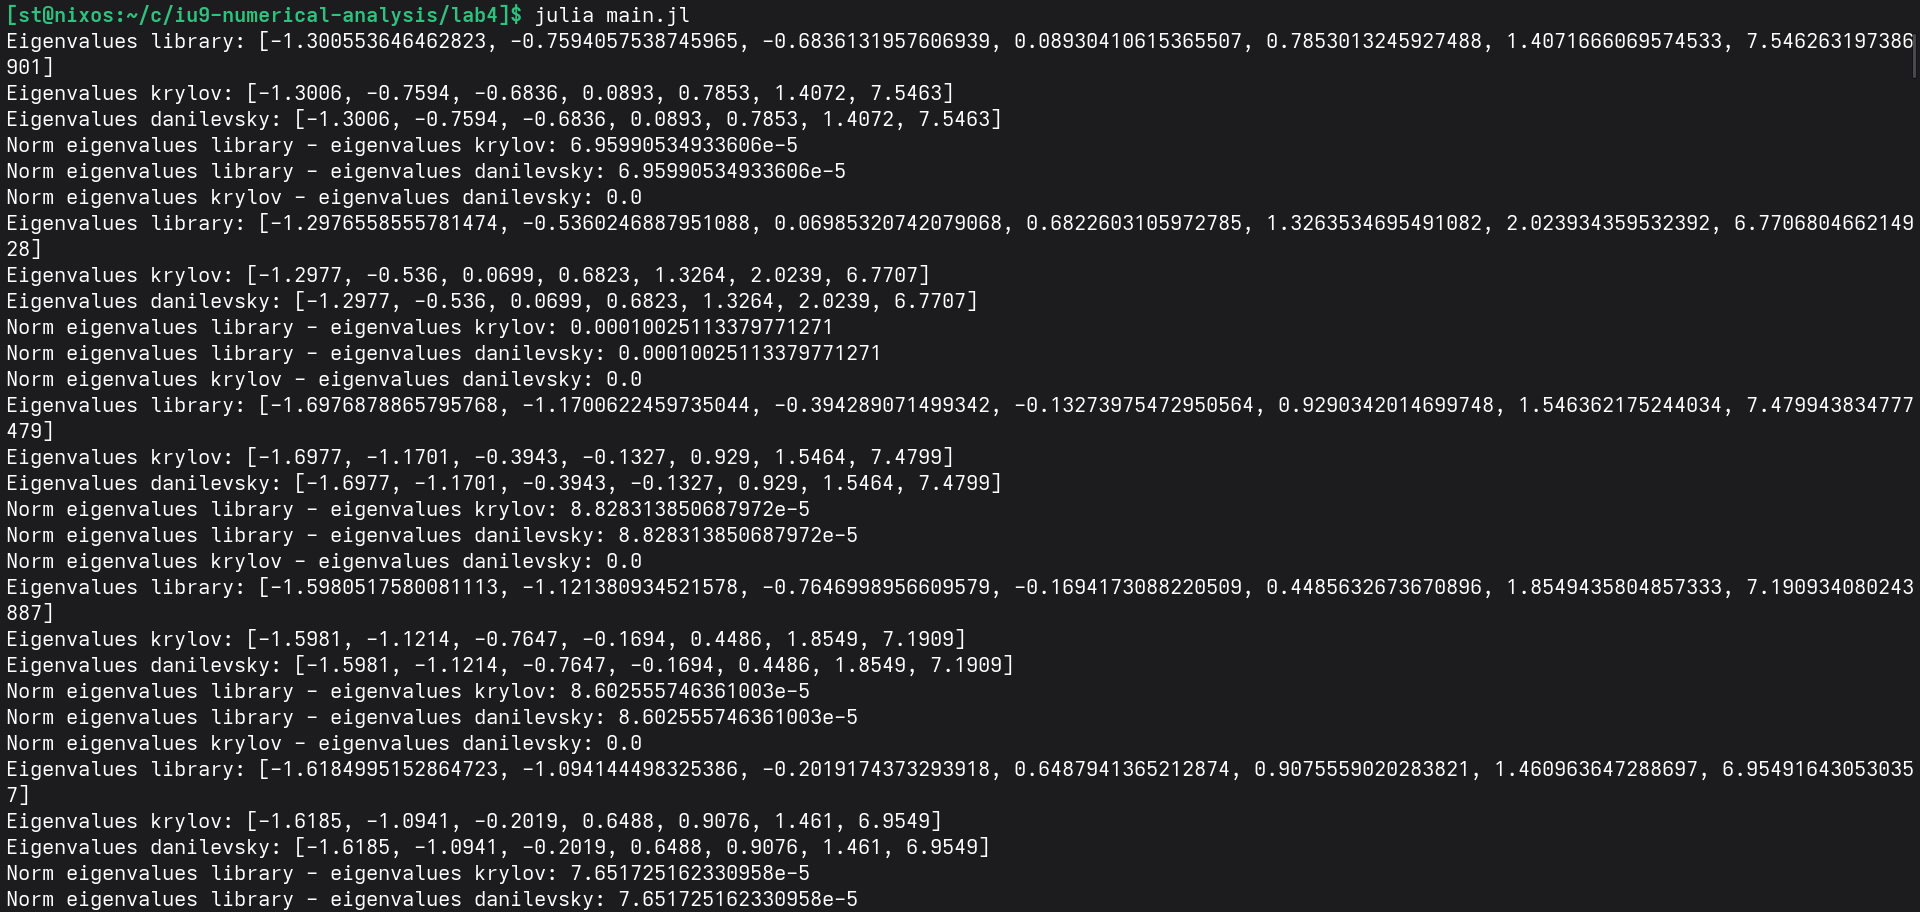
\includegraphics[width=0.8\textwidth]{img2}
\caption{Результат}
\label{fig:img2}
\end{figure}

\clearpage
\section{Выводы}\label{Sect::fin}

Результатом выполнения данной лабораторной работы является реализация метода
Крылова, позволяющего находить собственные значения матрицы, а также сравнение с
методом Данилевского.

\end{document}
